%Discovery Notes(up to 4 pages, this is approx. 3000 words) Discovery notes report biologically interesting discoveries using computational techniques.

%Application Notes (up to 2 pages; this is approx. 1300 words or 1000 words plus one figure) Applications Notes are short descriptions of novel software or new algorithm implementations, databases and network services (web servers, and interfaces). 

\documentclass{bioinfo}
\copyrightyear{}
\pubyear{}
%\firstpage{}
\usepackage{amsmath, amssymb}
\usepackage{natbib}
\usepackage{tikz}
\usepackage{pgfplots}
%\pgfplotsset{width=7cm,compat=1.5.1} 
\pgfplotsset{width=7cm} 
\usepackage[
   colorlinks=true, linkcolor=red, 
   citecolor=blue, urlcolor=blue
 ]{hyperref} 
 
\usepackage{txfonts}
%  $$$: 
%\usepackage[subscriptcorrection]{mtpro}
%\usepackage[mtphrb]{mtpams}
%\usepackage[mtpcal, mtpfrak]{mtpb}
%
\newcommand{\bA}{\textsf{\textit{A}}}
\newcommand{\bC}{\textsf{\textit{C}}}
\newcommand{\bG}{\textsf{\textit{G}}}
\newcommand{\bT}{\textsf{\textit{T}}}
%
%
% -----------------------------------------------------------
%
\begin{document}
\title[AID hotspots]{Constitution Analysis} 
 \author[I. T. Silva~\textit{et~al}]{%
     Israel T. Silva\,$^{1,3,}$\footnote{to
  whom correspondence should be addressed}\ , 
  and
       Rafael A. Rosales\,$^2$
  }

 \address{$^{1}$Laboratory of Molecular Immunology, The Rockefeller 
     University, 1230 York Avenue, New York, NY 10065\\
     $^{2}$Departamento de Computa\c{c}\~ao e Matem\'atica,
     Universidade de S\~ao Paulo. Av. Bandeirantes, 3900,
     Ribeir\~ao Preto,  CEP 14049-901, SP, Brazil%\\
%     $^{3}$National Institute of Science and Technology in Stem Cell
%     and Cell Therapy and Center for Cell Based Therapy. Rua Cat\~ao
%     Roxo, 2501, Ribeir\~ao Preto, CEP 14051-140, SP, Brazil
}

\history{Received on XXXXX; revised on XXXXX; accepted on XXXXX}
\editor{Associate Editor: XXXXXXX}

\maketitle
\begin{abstract}
  \section{Motivation:}
  \section{Results:} 
  \href{https://github.com/someone/rich}{\texttt{https://github.com/someone/rich}}.
  \section{Contact:}
  \href{mailto:someone@somewhere.world}{\tt someone@somewhere.world}%,
\end{abstract}

\section{Introduction}
The genome is targeted by a sophisticated and highly coordinated series of molecular events.  Among these events, aberrant DNA methylation patterns in human malignancy \cite{pmid23326238}, somatic retrotransposition in human cancers \cite{pmid22745252}, AID-dependent chromosomal translocations (Klein, 2011) and HIV integration (Cohn, 2014), which arrives throughout DNA, are not randomly distributed but instead associated with chromosomal regions and contributes to disrupt the integrity of the genome and human disease.

As result, these regions represents a genomic context in which are associate with multiple underlying mechanisms. The motif-based sequence analysis is the starting point to aim potential binding site of cis-regulatory elements associated. Nevertheless, the inherent low signal/noise ratio in sequence-based motif discovery is a limitation to detect a nucleic acid sequence pattern that has some biological significance. Moreover, these events may recognise a structural feature, rather than a specific sequence motif.

Others approaches were introduced to detect functional regions using methods for computing sequence complexities \cite{pmid24533097,pmid21317142}. In these methods, the complexity is measured by the entropy which evaluates the randomness of DNA sequence. In particular, topological entropy has been applied to compute the complexity of introns, exons and promoter regions. Due to the finite sample and high-dimensionality problems, efforts aimed to overcome these problems are put forward \cite{pmid21317142}.

However, how exactly the pattern nucleotide composition could influence the selection of target site selection are not well understood. To further characterize at a genome-wide scale these regions, we introduce a new method to provide a quantitative measure of the differential spectra of $k$-mers (DNA 'words' of length $k$) inside target DNA.


%!TEX root = ../enrichment.tex
\begin{figure}
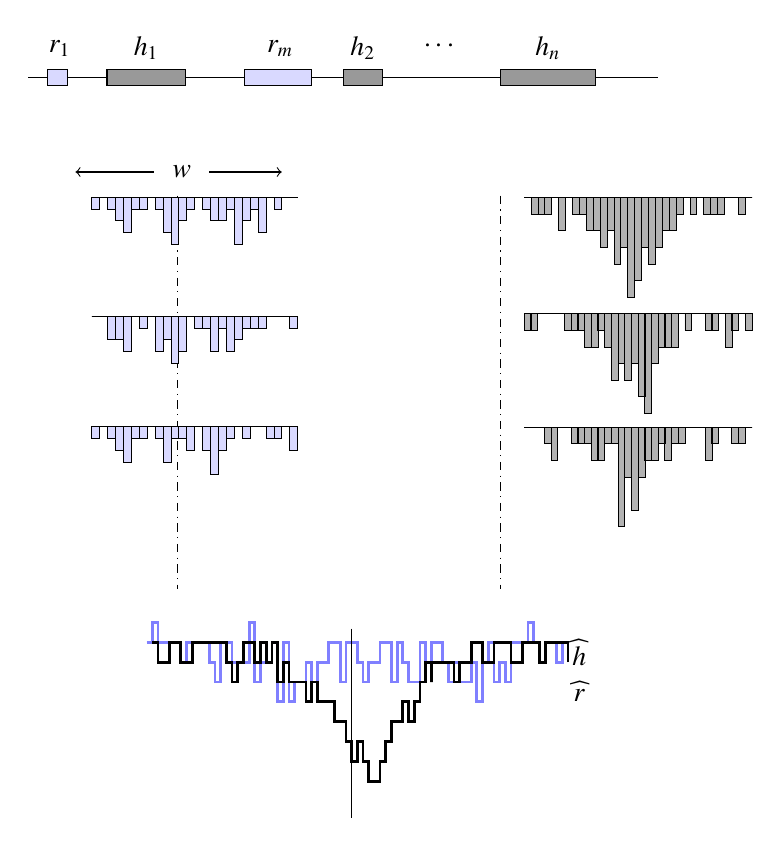
\begin{tikzpicture}
 \draw (0,0) -- (8,0);
 % hotspots
 \draw[fill=black!40] (1,-0.1) -- (2,-0.1) -- (2,0.1) -- (1,0.1) -- cycle;
 \draw[fill=black!40] (4,-0.1) -- (4.5,-0.1) -- (4.5,0.1) -- (4,0.1) -- cycle;
 \draw[fill=black!40] (6,-0.1) -- (7.2,-0.1) -- (7.2,0.1) -- (6,0.1) -- cycle;
 %
 \draw[fill=blue!15] (0.25,-0.1) -- (0.5,-0.1) -- (0.5,0.1) -- (0.25,0.1) -- cycle;
 \draw[fill=blue!15] (2.75,-0.1) -- (3.6,-0.1) -- (3.6,0.1) -- (2.75,0.1) -- cycle;
 % labels
 \node at (1.5,0.37)  {$h_1$};
 \node at (4.25,0.37)  {$h_2$};
 \node at (5.25,0.37)  {$\cdots$};
 \node at (6.6,0.37)  {$h_n$};
 \node at (0.4,0.37) {$r_1$};
 \node at (3.2,0.37) {$r_m$};
%
 \draw[<-] (0.6,-1.2) -- (1.6,-1.2);
 \draw[->] (2.3,-1.2) -- (3.22,-1.2);
 \node at (1.95,-1.2) {$w$};
% vertical lines   
 \draw[dashdotted] (1.9,-1.5) -- (1.9,-6.5);
 \draw[dashdotted] (6,-1.5) -- (6,-6.5);

\begin{axis}[
   at={(0.05\linewidth,-62pt)}, ybar, bar width=2.85pt, width=4.6cm, height=2.3cm,
   axis lines=none
   ]
\addplot[fill=blue!15, line width=0.35pt]%
 coordinates {
  (-2,-1) (-1,0) (0,-1) (1,-2) (2,-3) (3,-1) (4,-1) (5,0) (6,-1) (7,-3) (8,-4) (9,-2) (10,-1) (11,0) (12,-1) (13,-2) (14,-2) (15,-1) (16,-4) (17,-2) (18,-1) (19,-3) (20,0) (21,-1) (22,0) (23,0)
  };
\end{axis}
%
\begin{axis}[
   at={(0.05\linewidth,-145pt)}, ybar, bar width=2.85pt, width=4.6cm, height=2.3cm,
   axis lines=none
   ]
\addplot[fill=blue!15,  line width=0.35pt]%
 coordinates {
   (-2,-1) (-1,0) (0,-1) (1,-2) (2,-3) (3,-1) (4,-1) (5,0) (6,-1) (7,-3) (8,-1) (9,-1) (10,-2) (11,0) (12,-2) (13,-4) (14,-2) (15,-1) (16,0) (17,-1) (18,0) (19,0) (20,-1) (21,-1) (22,0) (23,-2)
 };
\end{axis}
%
\begin{axis}[
   at={(0.05\linewidth,-105pt)}, ybar, bar width=2.85pt, width=4.6cm, height=2.3cm,
   axis lines=none
   ]
\addplot[fill=blue!15,  line width=0.35pt]%
 coordinates {
   (-2,0) (-1,0) (0,-2) (1,-2) (2,-3) (3,-0) (4,-1) (5,0) (6,-3) (7,-2) (8,-4) (9,-3) (10,0) (11,-1) (12,-1) (13,-3) (14,-1) (15,-3) (16,-2) (17,-1) (18,-1) (19,-1) (20,0) (21,0) (22,0) (23,-1)
 };
\end{axis}
%   
%  
%
\begin{axis}[
   at={(0.5\linewidth,-83pt)}, ybar, bar width=2.5pt, width=4.95cm, height=3.1cm,
   axis lines=none
   ]
\addplot[fill=black!30, line width=0.35pt]%
 coordinates {
  (-1,0) (0,-1) (1,-1) (2,-1) (3,-0) (4,-2) (5,0) (6,-1) (7,-1) (8,-2) (9,-2) (10,-3) (11,-2) (12,-4) (13,-3) (14,-6) (15,-5) (16,-3) (17,-4) (18,-3) (19,-2) (20,-2) (21,-1) (22,0) (23,-1) (24, 0) (25,-1) (26,-1) (27,-1) (28,0) (29,0) (30,-1) (31,0)
  };
\end{axis}
%
\begin{axis}[
   at={(0.5\linewidth,-125pt)}, ybar, bar width=2.5pt, width=4.95cm, height=3.1cm,
   axis lines=none
   ]
\addplot[fill=black!30,  line width=0.35pt]%
 coordinates {
  (-1,-1) (0,-1) (1,0) (2,0) (3,-0) (4,-0) (5,-1) (6,-1) (7,-1) (8,-2) (9,-2) (10,-1) (11,-2) (12,-4) (13,-3) (14,-4) (15,-3) (16,-5) (17,-6) (18,-3) (19,-2) (20,-2) (21,-2) (22,0) (23,-1) (24, 0) (25,0) (26,-1) (27,-1) (28,0) (29,-2) (30,-1) (31,0) (32,-1)
 };
\end{axis}
%
\begin{axis}[
   at={(0.5\linewidth,-166pt)}, ybar, bar width=2.5pt,width=4.95cm, height=3.1cm,
   axis lines=none
   ]
\addplot[fill=black!30,  line width=0.35pt]%
 coordinates {
  (-2,0) (-1,0) (0,0) (1,-1) (2,-2) (3,-0) (4,-0) (5,-1) (6,-1) (7,-1) (8,-2) (9,-2) (10,-1) (11,-1) (12,-6) (13,-3) (14,-5) (15,-3) (16,-2) (17,-2) (18,-1) (19,-2) (20,-1) (21,-1) (22,0) (23, 0)  (24, 0) (25,-2) (26,-1) (27,0) (28,0) (29,-1) (30,-1) (31,0)
 };
\end{axis}
% The ``sum'' of all histograms
\begin{axis}[
   width=8cm, height=4cm,
   at={(0.08\linewidth,-260pt)},
   hide x axis,
   hide y axis,
   mark size = 0pt
   ]
\addplot+[const plot, draw=blue!50, line width=1pt]%
 coordinates {
  (-10,0) (-9,1) (-8,-0) (-7,-0) (-6,0)  
  (-5,0) (-4,-1) (-3,-0) (-2,-0) (-1,0)  (0,0)
  (1,-1) (2,-2) (3,-0) (4,-0) (5,-1) 
  (6,-1) (7,-1) (8,1) (9,-2) (10,-1) 
  (11,-1) (12,-0) (13,-3) (14,0) (15,-3) 
  (16,-2) (17,-2) (18,-1) (19,-2) (20,-1) 
  (21,-1) (22,0) (23, 0) (24,-2) (25,0) 
  (26,0) (27,-1) (28,-2) (29,-1) (30,-1)
  (31,0) (32,0) (33,-2) (34,0) (35,-1)
  (36,-2) (37,-2) (38,0) (39,-1) (40,-1)
  (40,-0) (41,-0) (42,-1) (43,-2) (44,-1) 
  (45,-2) (46,-2) (47,-1) (48,-3) (49,-1) 
  (50,0) (51,-2) (52,-1) (53,-2) (54,0)
  (55,0) (56,0) (57,1) (58,0) (59,-1)
  (60,0) (61,0) (62,-1) (63,0) (64,-1)

 };
\addplot+[const plot, draw=black, line width=1pt]%
 coordinates {
   (-9,0) (-8,-1) (-7,-1) (-6,0) (-5,0) 
  (-4,-1) (-3,-1) (-2,-0) (-1,-0) (0,0) 
  (1,0) (2,0) (3,0) (4,-1) (5,-2) 
  (6,-1) (7,0) (8,0) (9,-1) (10,0) 
  (11,-1) (12,-0) (13,-2) (14,-1) (15,-2) 
  (16,-2) (17,-2) (18,-3) (19,-2) (20,-3) 
  (21,-3) (22,-3) (23, -4) (24,-4) (25,-5) 
  (26,-6) (27,-5) (28,-6) (29,-7) (30,-7)
  (31,-6) (32,-5) (33,-4) (34,-4) (35,-3)
  (36,-4) (37,-3) (38,-2) (39,-1) (40,-2)
  (40,-1) (41,-1) (42,-1) (43,-1) (44,-2) 
  (45,-1) (46,-1) (47,0) (48,0) (49,-1) 
  (50,-1) (51,0) (52,0) (53,0) (54,-1) 
   (55,-1) (56,0) (57,0) (58,0) (59,-1)
  (60,0) (61,0) (62,0) (63,0) (64,-1)
 };
\end{axis}
\node at (7, -7.3) {$\widehat h$};
\node at (7,-7.8) {$\widehat r$};
\draw[] (4.11,-7) -- (4.11,-9.4);

\end{tikzpicture}
\label{fig:methodscheme}
\caption{The method}
\end{figure}



\section{Methods}
We specialise to regions conforming to viral insertion hotspots, but the method is clearly not restricted to this application. Insertion hotspots are detected by using scan statistics as described in \cite{IRAMM}. Let $\{h_1, \ldots, h_n\}$, bet a set of insertion hotspots and let $w$ be the length (in base pairs) of the longest such segments. The coordinates of all the hotspots were extended at bot extremes such to match exactly this length. The resulting set of segments were partitioned into $k$ evenly spaced bins of length $\rho = w/k$. Denote by $h_{ij}$, $1 \leq j \leq k$, the $j$th interval of the $i$th segment. Let $\{r_1, \ldots, r_n\}$, be a set segments of width $w$, uniformly distributed along the genome but with no intersection with $h_{i}$, $1 \leq i \leq n$. Also, denote by $r_{ij}$ the $j$th interval of the $i$th segment.

%$$ 
% \xi_p = \frac{1}{nm}\frac{k}{w} 
%   \sum_{i=1}^m\sum_{j=1}^{n} 1_{\{\xi_{ij} \in I_p\}}
%$$

Let $\mathcal A = \{\sf A, C, G, T\}$ and $\mathcal S \in \mathcal A^\ell$, be a string of length $\ell \leq \rho$. Let $\xi_{ij}$ and $\eta_{ij}$ for $1 \leq i \leq n$, $1 \leq j \leq k$, be random variables defined as 
\[
   \xi_{ij} = %\mathbb 1_{\{\mathcal S \in h_{ij}\}} =
    \begin{cases}
     1, & \text{if } \mathcal S \in h_{ij}\\
     0, &\text{otherwhise}
    \end{cases}
    \quad\text{and}\quad
   \eta_{ij} = %\mathbb 1_{\{\mathcal S \in r_{ij}\}} =
       \begin{cases}
     1, &\text{if } \mathcal S \in r_{ij}\\
     0, &\text{otherwhise}
    \end{cases}.
\]
Consider the counts
\[
   X_j = \sum_{i=1}^n \xi_{ij}, \qquad 
   Y_j = \sum_{i=1}^n \eta_{ij}
\]
that is $X_j$ and $Y_j$ reccord the number of times that $\mathcal S$ occurs along each bin of a hotspot and a randomly chosen region respectively. In order to asses if the distribution of $\mathcal S$ varies differently across the bins of a hotspot region, we may consider the following test. Let
\[
  X^{2} = \sum_{j=1}^k (X_{j}-Y_{j})^2/Y_{j}.
\]
Provided the number of counts in each of the $k$ bins is sufficiently large, $X^{2}$ is a $\chi^{2}$ random variable with $k-1$ degrees of freedom. This provides then the sampling distribution to perform Pearson's $\chi^{2}$ test for a $2\times k$ contingency table, with $H_{0}$ and $H_{a}$ ...


\bibliographystyle{natbib}
\scriptsize{
   \bibliography{rich}
\normalsize
}
\end{document}
